% /01_draft/chapter4/chapter4_v2.tex

\chapter{評価実験}

\section{データセット}

IFOR手法の開発において,地域間のドメインシフトを考慮したモデルの性能評価は重要である.
このドメインシフトを実現するため,学習用と評価用のデータセットを異なる地域から選定した.
具体的には,学習用データセットとして南米の野生動物画像を集めたWCS Camera Traps (WCS) \cite{wcs}を,
評価用データセットとして北米の野生動物画像から構成されるCaltech Camera Traps (CCT) \cite{cct}をそれぞれ採用した.

本実験では,提案手法の有効性を多角的に検証するため,各データセットにおいて赤外線画像と可視光画像それぞれから構成される2種類のデータセットを作成した.
このアプローチにより,提案手法が赤外線画像特有の性質に対して有効であるのか,
あるいは,赤外線画像や可視光画像を問わず広義の画像分類に対して有効であるのかを検証することが可能となる.

データセットの前処理では,各画像を赤外線画像と可視光画像に分類し,
アノテーションとして提供されているバウンディングボックスに基づいてクロッピングを行い,動物が存在している領域を切り出した.
バウンディングボックスに基づき動物領域が切り出された例を図 \ref{fig:cropping}に示す.
% 
\begin{figure}[tbp]
  \centering
  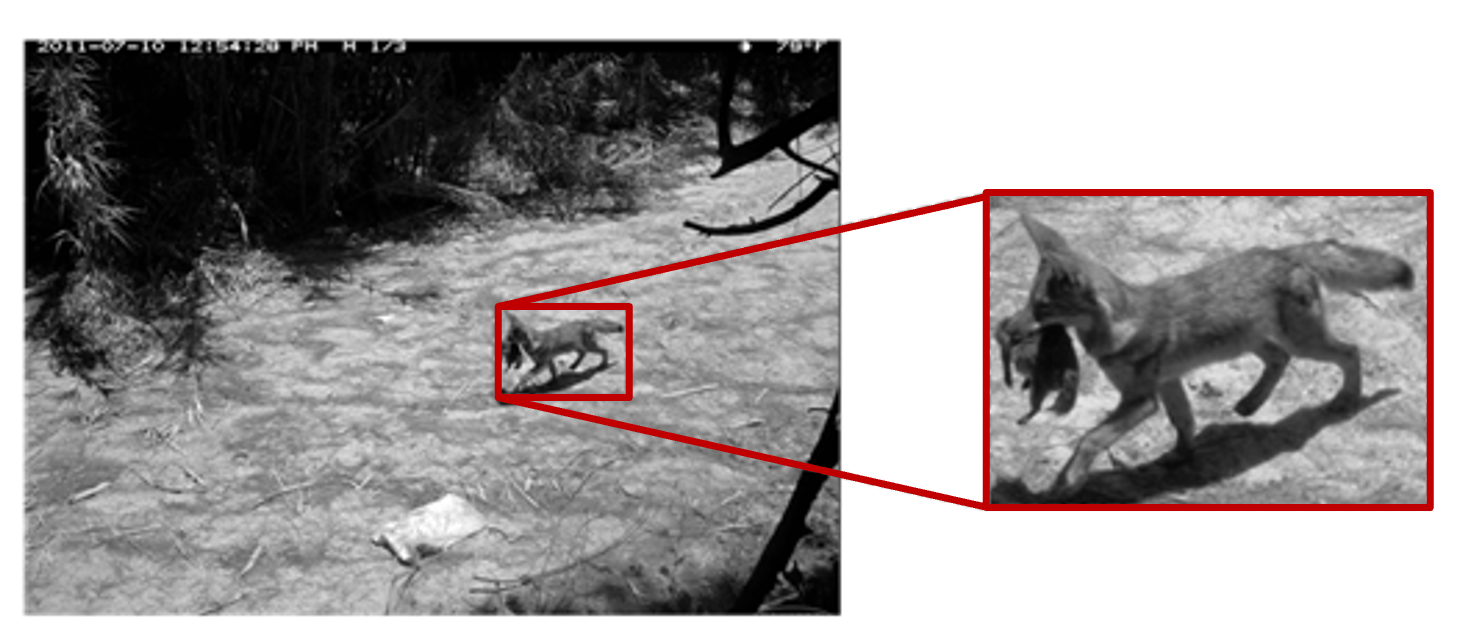
\includegraphics[width=\linewidth, keepaspectratio]{image/cropping.png}
  \caption{バウンディングボックスによって動物領域が切り出されている例}
  \label{fig:cropping}
\end{figure}
% \begin{figure}[tbp]
%   \centering
%   \begin{subfigure}[b]{0.45\linewidth}
%     \centering
%     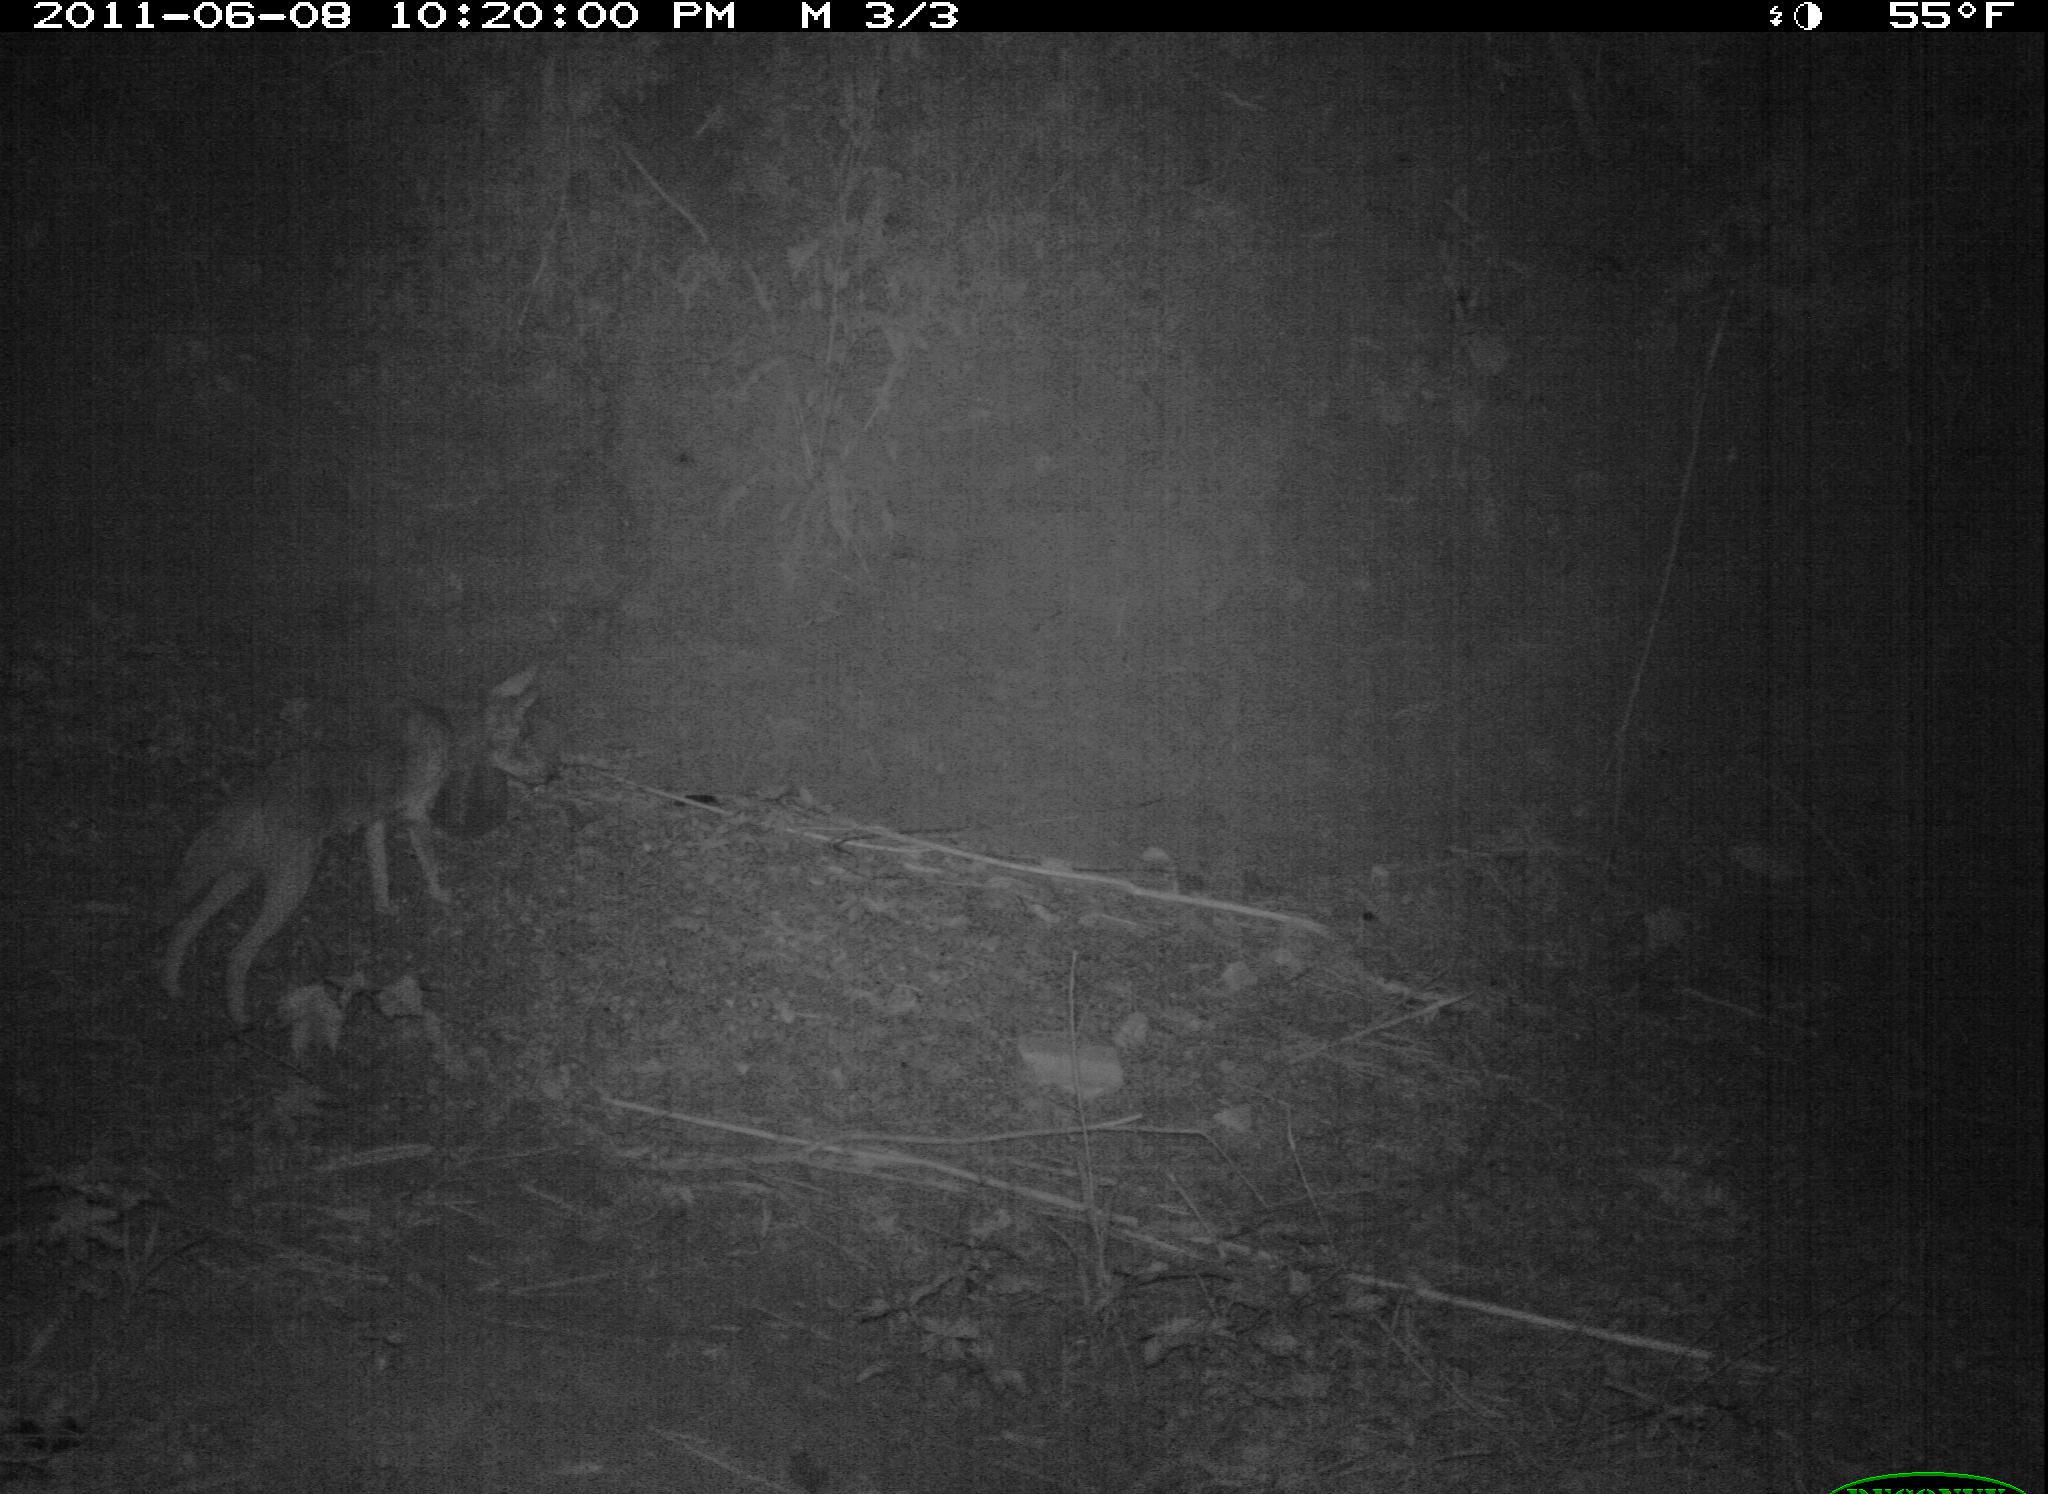
\includegraphics[height=0.9\linewidth, keepaspectratio]{image/coyote_full.png}
%     \caption{原画像}
%     \label{fig:fullimg}
%   \end{subfigure}
%   \hfill
%   \begin{subfigure}[b]{0.45\linewidth}
%     \centering
%     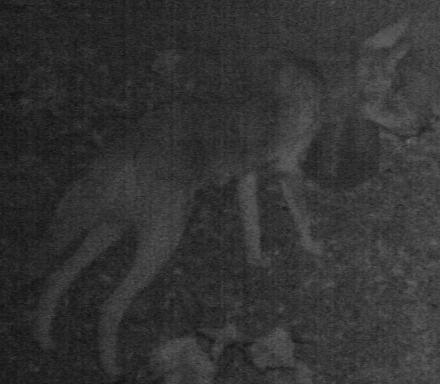
\includegraphics[height=0.9\linewidth, keepaspectratio]{image/coyote_cropped.png}
%     \caption{クロッピングされた画像}
%     \label{fig:croppedimg}
%   \end{subfigure}
%   \caption{バウンディングボックスによって}
%   \label{fig:cropbybbox}
% \end{figure}
% 
その後,実験の公平性を確保するため,赤外線画像と可視光画像による学習用データセット間でクラス数と画像枚数を同数に統一した.
同様に,評価用データセットについてもクラス数と画像枚数を同一に設定した.
具体的には,学習用データセットは28クラス,各クラス約500枚ずつの合計14,000枚の画像で構成され,
評価用データセットは11クラス,各クラス100枚ずつの合計1,100枚の画像により構成される.
これらの処理により,学習用データセットとして赤外線画像及び可視光画像による2種類の WCS データセット,
評価用データセットとして赤外線画像及び可視光画像による2種類の CCT データセットの計4種類のデータセットを作成した.
ただし,画像の前処理過程において,学習用データセットでは赤外線画像が13,687枚,可視光画像が13,812枚と若干の不均衡が生じたが,
この僅かな差異は実験結果に重大な影響を及ぼさないと考えられる.
これらの前処理によって作成された各データセットの詳細を表 \ref{tbl:wcs}及び表 \ref{tbl:cct}に示す.

\begin{table}[tbp]
  \centering
  \caption{学習用データセット (WCS Camera Traps) データセットの詳細}
  \label{tbl:wcs}
  \begin{tabular}{c|c|c}
      \hline
      動物種                    & 赤外線画像(枚) & 可視光画像(枚) \\ \hline\hline
      acryllium vulturinum     & 500          & 500          \\
      aepyceros melampus       & 500          & 500          \\
      bos taurus               & 500          & 500          \\
      capra aegagrus           & \textbf{337} & 500          \\
      cephalophus nigrifrons   & 500          & 500          \\
      crax rubra               & 500          & 500          \\
      cuniculus paca           & 500          & \textbf{495} \\
      dasyprocta punctata      & 500          & 500          \\
      equus quagga             & 500          & 500          \\
      giraffa camelopardalis   & 500          & 500          \\
      leopardus pardalis       & 500          & 500          \\
      loxodonta africana       & 500          & 500          \\
      madoqua guentheri        & 500          & 500          \\
      mazama americana         & 500          & 500          \\
      mazama temama            & 500          & 500          \\
      meleagris ocellata       & 500          & 500          \\
      mitu tuberosum           & 500          & 500          \\
      nasua narica             & \textbf{350} & 500          \\
      panthera onca            & 500          & 500          \\
      papio anubis             & 500          & 500          \\
      pecari tajacu            & 500          & 500          \\
      phacochoerus africanus   & 500          & \textbf{317} \\
      psophia leucoptera       & 500          & 500          \\
      puma concolor            & 500          & 500          \\
      syncerus caffer          & 500          & 500          \\
      tapirus terrestris       & 500          & 500          \\
      tayassu pecari           & 500          & 500          \\
      urocyon cinereoargenteus & 500          & 500          \\ \hline\hline
      合計                      & 13,687       & 13,812       \\ \hline
  \end{tabular}
\end{table}

\begin{table}[tbp]
  \centering
  \caption{評価用 (Caltech Camera Traps) データセットの詳細}
  \label{tbl:cct}
  \begin{tabular}{c|c|c}
      \hline
      動物種       & 赤外線画像(枚) & 可視光画像(枚) \\ \hline\hline
      bird        & 100      & 100       \\
      bobcat      & 100      & 100       \\
      cat         & 100      & 100       \\
      coyote      & 100      & 100       \\
      deer        & 100      & 100       \\
      dog         & 100      & 100       \\
      fox         & 100      & 100       \\
      opossum     & 100      & 100       \\
      rabbit      & 100      & 100       \\
      skunk       & 100      & 100       \\
      squirrel    & 100      & 100       \\ \hline\hline
      合計         & 1,100    & 1,100     \\ \hline
  \end{tabular}
\end{table}

\section{未登録クラスの検出に対する提案手法の評価}
\label{sec:detect}

\subsection{実験条件}

本実験では,IFORフレームワークにおける特徴抽出器の有効性を評価するため,異なる性質を持つCNNベース及びViTベースの特徴抽出器について検証を行う.
CNNベースのモデルには,18層の深さと約1,170万のパラメータを有するResNet18 \cite{resnet}を採用した.
ResNet18は,小規模から中規模のデータセットに対して,十分な分類性能を維持しながら効率的な処理が可能なアーキテクチャとして知られている.
一方,ViTベースのモデルとして,Data-efficient image Transformers (DeiT) \cite{deit} の最軽量モデルであるDeit-Tiを利用した.
このアーキテクチャは,約500万のパラメータを有し,モデルのスケールと計算効率の両立を実現している.
DeiTは,入力画像を16$\times$16 pix.のパッチに分割し,自己注意機構を適用することによって特徴抽出を行う.
これらのモデルはImageNetデータセットまたはFDSLを用いた事前学習が適用されており,
それぞれの転移学習手法がIFORフレームワークのモデル性能に与える影響について検証することが可能である.

IFORでは,特定の地域に生息する野生動物の画像を大量に収集することが困難な状況を想定している.
このような実世界での制約を考慮し,本研究で用いるデータ設定は極めて厳しい条件である5-Way, 1-Shot問題として定義した.
本実験設定は,新規地域において,わずか1クラスあたり1枚の画像を収集するだけでモデルが利用できる状況を仮定しており,システムの初期導入時に想定される最小限のデータ条件である.

学習の際には,各エピソードにつき学習用データセットから10クラスがランダムに選択される.
このうち5クラスは登録クラス,残りの5クラスは未登録クラスとして設定される.
サポートセットとクローズドクエリセットには登録クラスからのデータのみが使用され,オープンクエリセットには未登録クラスからのデータが割り当てられる.

メタ学習の各学習エピソードでは,学習用データセットからサポートセットとして1クラスにつき1枚,クローズドクエリセットとして1クラスにつき15枚,
オープンクエリセットとして1クラスにつき15枚の画像を用いる.
これに加えて,75枚の画像がベースデータとしてランダムに選択される.
最適化関数にはAdamを採用し,入力画像は224$\times$224 pix. にリサイズを行った.
学習エピソードの総数は30,000エピソードとし,学習過程でモデルが局所最適解に陥るのを防ぐため,10,000エピソード時と20,000エピソード時に学習率を0.1倍ずつ減少させた.
本実験では,様々な転移学習手法や特徴抽出器の組み合わせを検証するため,各実験設定における最適な初期学習率が異なる.
そこで,初期学習率を$10^{-6}$から$10^{-2}$まで10倍ずつ増加させて最適な学習率の探索を行い,最も高い精度が得られた重みを採用した.

評価実験では,新規地域で収集された限られたデータによる実運用を想定し,評価用データセットを用いて実用的な条件下でのモデルの性能評価を行った.
本実験は5-Way, 1-Shot問題として定義され,5つのクラスにそれぞれ1枚ずつ,合計5枚のサポートセットによる評価を行った.
クエリセットも学習時と同様に,サポートセットと同一の5クラスを登録クラス,サポートセットと異なる5クラスを未登録クラスとして設定した.
具体的な評価手順は次の通りである.

まず,評価用データセットからランダムに選択された5つのクラスから,それぞれ1枚の画像をプロトタイプとしてモデルに登録する.
次に,特徴抽出器によって得られたクローズドクエリセットの特徴ベクトルを距離が最も近いプロトタイプのクラスへと分類し,正しく分類できた割合に基づいて分類精度を測定する.
オープンクエリデータを未登録クラスとして検出するモデルの能力は,AUROC (Area Under the Receiver Operating Characteristic Curve) 指標により評価される.
AUROCは,クエリデータとプロトタイプ間の距離スコアに対する閾値を変化させた際の,偽陽性率 (False Positive Rate, FPR) と
真陽性率 (True Positive Rate, TPR) の関係をプロットしたグラフの曲線下の面積として定義されている.
この指標は値が100\%に近づくほど,未登録クラスに対する検出精度が高いことを示す.
% この指標は,0から100の範囲をとり,100に近いほど未登録クラスに対する検出精度が高いことを示す.
ここで,TPRはオープンクエリデータを正しく未登録クラスとして検出できたサンプルの割合を表し,FPRは登録クラスを誤って未登録クラスとして検出したサンプルの割合を示す.
評価用データセットからのクラス選択が特定のクラスに集中することで生じるバイアスなどを排除し,実験結果の妥当性を担保するため,この評価手順を10,000エピソードにわたり実施した.

\subsection{実験結果及び考察}

本実験では,異なる特徴抽出器であるResNet18とViTについて,ImageNet転移学習,フラクタル転移学習,転移学習なしの3つの実験条件で比較を行った.
なお,転移学習なしの条件では,モデルの重みをランダムに初期化し,WCSデータセットを用いたメタ学習によりモデルのパラメータをスクラッチから更新した.
これらの条件下におけるIFORに対するそれぞれの実験結果を表 \ref{tbl:exp1}に示す.
% 
\begin{table}[tbp]
  \centering
  \caption{IFORに対する各特徴抽出器と転移学習の組み合わせによる実験結果}
  \label{tbl:exp1}

  \begin{tabular}{cc||c|c|c|c|c|c}
      \hline
      \multicolumn{2}{c||}{学習方法}            & \multicolumn{6}{c}{メタ学習 (PEELER)}                        \\ \hline
      \multicolumn{2}{c||}{特徴抽出器}           & \multicolumn{3}{c|}{ResNet18} & \multicolumn{3}{c}{ViT}     \\ \hline
      \multicolumn{2}{c||}{転移学習}            &  ImageNet  &  FDSL  &  なし   &   ImageNet    & FDSL & なし  \\ \hline\hline
      \multirow{2}{*}{赤外線画像} & 分類精度 (\%) &    45.8    &  38.8  &  38.6  & \textbf{51.0} & 36.5 & 36.2 \\
                                & AUROC (\%)   &    58.4    &  54.3  &  56.3  & \textbf{61.0} & 54.4 & 54.5 \\ \hline
      \multirow{2}{*}{可視光画像} & 分類精度 (\%) &    53.0    &  32.8  &  33.2  & \textbf{60.2} & 32.7 & 31.4 \\
                                & AUROC (\%)   &    60.8    &  55.2  &  54.3  & \textbf{67.8} & 54.6 & 53.9 \\ \hline
  \end{tabular}
\end{table}
% 
表 \ref{tbl:exp1}に示す全ての実験において,モデルの学習にメタ学習を適用した.
各特徴抽出器に対する実験結果から,赤外線画像の分類においてViTがResNet18よりも高い精度を示すことが明らかとなった.
ただし,転移学習なしの条件下では,ViTはResNet18よりも低い精度を示した.
これは,転移学習を適用しない場合,ViTよりもCNNベースのモデルの方が優れた性能を示すという従来の知見 \cite{vit}と一致する結果である.

表 \ref{tbl:exp1}より,ResNet18とViTの両モデルにおいて,ImageNetを用いた転移学習が赤外線画像と可視光画像の双方のデータセットに対して最も高い精度を示した.
FDSLによる転移学習は,転移学習なしの場合と比較して,赤外線画像と可視光画像ともに精度をわずかに改善しただけであった.
このような傾向が見られた背景として,フラクタル画像のドメインが自然画像とは異なることから,赤外線画像や可視光画像の動物分類タスクにおいて効果が限定的となった可能性が考えられる.
一方で,FDSLを用いた先行研究では,自然画像で構成されるCIFAR10データセットにおいて,FDSLによって転移学習されたモデルがImageNetを用いて転移学習したモデルを凌駕する性能を示している \cite{fdsl}.
この知見から,FDSLを赤外線画像分類に効果的に適用するためには,自然画像で構成されたデータセットによるファインチューニングが必要である可能性を示唆している.

本研究では,IFORフレームワークにおけるメタ学習の影響も検証しており,その結果を表 \ref{tbl:exp2}に示す.
% 
\begin{table}[tbp]
  \centering
  \caption{ImageNet転移学習を用いた場合のViTによる各学習方法のIFORに対する実験結果}
  \label{tbl:exp2}
  \begin{tabular}{cc||c|c|c}
      \hline
      \multicolumn{2}{c||}{特徴抽出器}          &          \multicolumn{3}{c}{ViT}                \\ \hline
      \multicolumn{2}{c||}{転移学習}            &          \multicolumn{3}{c}{ImageNet}           \\ \hline
      \multicolumn{2}{c||}{学習方法}            & メタ学習 (PEELER)  & 従来法(ミニバッチ学習) & なし  \\ \hline\hline
      \multirow{2}{*}{赤外線画像} & 分類精度 (\%) &  \textbf{51.0}   &        39.9          & 39.6  \\
                                & AUROC (\%)   &  \textbf{61.0}   &        53.3          & 55.0  \\ \hline
  \end{tabular}
\end{table}
% 
本実験では,ImageNetで事前学習されたViTモデルを特徴抽出器として使用し,WCSデータセットを用いて動物分類タスクのためにファインチューニングを行った.
なお,「学習方法」によってファインチューニングのアプローチが異なることに注意が必要である.
メタ学習の場合,分類ヘッドを使用せずに各エピソードで特徴抽出器をファインチューニングしている.
具体的には,特徴空間におけるサポートセットとクローズドクエリセット間,並びに,サポートセットとオープンクエリセット間の距離に基づいて特徴抽出器のパラメータを更新した.
一方,従来の学習手法であるミニバッチ学習の場合,28個のクラスノードを持つ分類ヘッドを用いて,特徴抽出器を含む全ての層を更新した.
この手法は,ImageNetを用いた事前学習と,ターゲットタスクデータセットを用いたミニバッチ学習を組み合わせた一般的な学習アプローチであり,本研究におけるベースラインとして位置付けされる.
また,学習なしの場合,ImageNetで事前学習された重みをWCSデータセットでの追加学習を行わずに使用した.
本研究の評価方法は特徴空間上の距離に基づいて分類を行うため,一般的な転移学習で行われる重みの凍結や分類ヘッドの再学習は不要であった.
メタ学習との公平な評価条件を確保するため,学習に使用する画像枚数を統一し,学習エポック数を690エポックに設定した.
初期学習率は$10^{-6}$から$10^{-2}$まで10倍ずつ増加させて最適値の探索を行い,学習過程において,学習率は230エポックごとに0.1倍ずつ減少させた.
IFORフレームワークにおけるモデルの性能評価は,評価用データセットを用いて10エポックごとに検証を行い,得られた最も高い精度を最終的な実験結果として採用した.

表 \ref{tbl:exp2}は,IFORフレームワークにおいて,ミニバッチ学習や学習なしの条件と比較して,メタ学習が分類精度とAUROCの両方を顕著に改善したことを示している.
ミニバッチ学習は,学習なしの条件と比較して分類精度をわずかに向上させたものの,AUROCは低下する結果となった.
% この結果は,未登録クラスの検出を考慮せずに28クラスの赤外線画像を分類する手法がAUROCの低下につながったことを示しており,IFORにおけるメタ学習の有効性を裏付けている.
この結果は,従来の学習手法であるミニバッチ学習が28クラスの識別に特化した特徴抽出器の学習を行うため,特徴空間上の各クラスの分布が未登録クラスの検出に適さない形で最適化されたことを示唆している.
一方,メタ学習では特徴空間における距離関係を直接的に学習することにより,登録クラスの分類と未登録クラスの検出を同時に考慮した特徴表現の獲得が可能となり,結果としてAUROCの向上につながったと考えられる.

% 結論として,本研究は赤外線画像を用いたタスク分類の複雑さを探究し,色情報の欠如による困難さの増大を強調している.
% 可視光画像と赤外線画像に対する分類性能の比較分析により,赤外線画像に関連する課題の高さが確認された.
本実験を通じて,赤外線画像による動物分類タスクの複雑性が明らかとなり,特に色情報の欠如に起因する課題の重要性が示された.
さらに,可視光画像と赤外線画像の分類性能の比較分析により,赤外線画像特有の課題の顕著さが確認された.

また,本実験ではIFORにおける基盤モデルを用いた意味的な特徴抽出の有効性についても検証を行った.
本実験で用いる特徴抽出器のモデル構造には,ViTの標準的なモデルサイズであるViT-Baseを採用した.
基盤モデルについては,ViTベースのCLIPモデルとしてViT-B/16を利用し,以降,これをCLIPと表記する.
一方,比較対象であるテキストを用いた学習が行われていないViTはViT-Baseと表記する.
これらのアーキテクチャは,約8,600万のパラメータを有しており,入力画像を16$\times$16 pix.のパッチに分割し特徴抽出が行われる.
CLIPはインターネットを介して収集された約4億組の画像とテキストのペアから構成されるWebImageText (WIT) という大規模データセットを使用して事前学習されている.
一方で,ViT-BaseはImageNet-1kの拡張版データセットであり,21,000クラスを含むImageNet-21kを用いて事前学習が行われている.

表 \ref{tbl:exp3}にCLIPの追加学習の有無が赤外線画像の分類類性能に与える影響を示している.
% 
\begin{table}[tbp]
  \centering
  \caption{IFORにおける基盤モデルの追加学習の有無による分類性能の実験結果}
  \label{tbl:exp3}

  \begin{tabular}{cc||c|c|c|c}
      \hline
      \multicolumn{2}{c||}{特徴抽出器}      & \multicolumn{2}{c|}{CLIP} & \multicolumn{2}{c}{ViT-Base} \\ \hline
      \multicolumn{2}{c||}{転移学習}       &  \multicolumn{2}{c|}{WIT}  & \multicolumn{2}{c}{ImageNet-21k} \\ \hline
      \multicolumn{2}{c||}{学習方法}       & メタ学習 (PEELER) &   なし   & メタ学習 (PEELER) &    なし    \\ \hline\hline
      \multirow{2}{*}{赤外線画像} & 分類精度 (\%) &       58.6      &   36.7   &  \textbf{61.1}  &    39.8    \\
                                & AUROC (\%)   &       64.8      &   54.9   &  \textbf{68.6}  &    58.0    \\ \hline
  \end{tabular}
\end{table}
% 
実験結果から,追加学習の有無に関わらずIFORにおけるCLIPの性能はViT-Baseに劣ることが明らかとなった.
本実験では,特徴空間上での距離に基づいた評価を行ったが,先行研究 \cite{clip}ではテキストエンコーダを用いた分類を行っている.
CLIPの学習ではテキストの特徴ベクトルと画像の特徴ベクトルとの類似度に基づき分類を行っているため,画像の特徴ベクトルのみを用いた分類には不向きである可能性がある.
この事実から,CLIPをIFORフレームワークに効果的に適用するためには,テキストエンコーダを用いた類似度計算が必要である可能性を示唆している.

\section{未登録クラスの多クラス分類に対する損失関数の評価}

\subsection{実験条件}

未登録の動物種に対する分類精度の評価に際し,本実験では新たな評価手法を導入した.
\ref{sec:detect} 節の実験の評価時には,登録クラスから得られるプロトタイプのみを用いて分類精度を求めていたが,
本実験では登録クラスのプロトタイプに加えて,未登録クラスから算出されるプロトタイプを用いて未登録クラスに対する分類精度も測る.
ここで,登録クラスから構成されたサポートセットをクローズドサポートセット (closed-support set) と呼び,それから得られるプロトタイプをクローズドプロトタイプ (closed-prototype) と呼ぶ.
同様に,未登録クラスから構成されたサポートセットをオープンサポートセット (open-support set) と呼び,それから得られるプロトタイプをオープンプロトタイプ (open-prototype) と呼ぶ.
図 \ref{fig:openprototype}にクローズドプロトタイプとオープンプロトタイプを用いた評価方法の概要を示している.
% 
\begin{figure}[tbp]
  \centering
  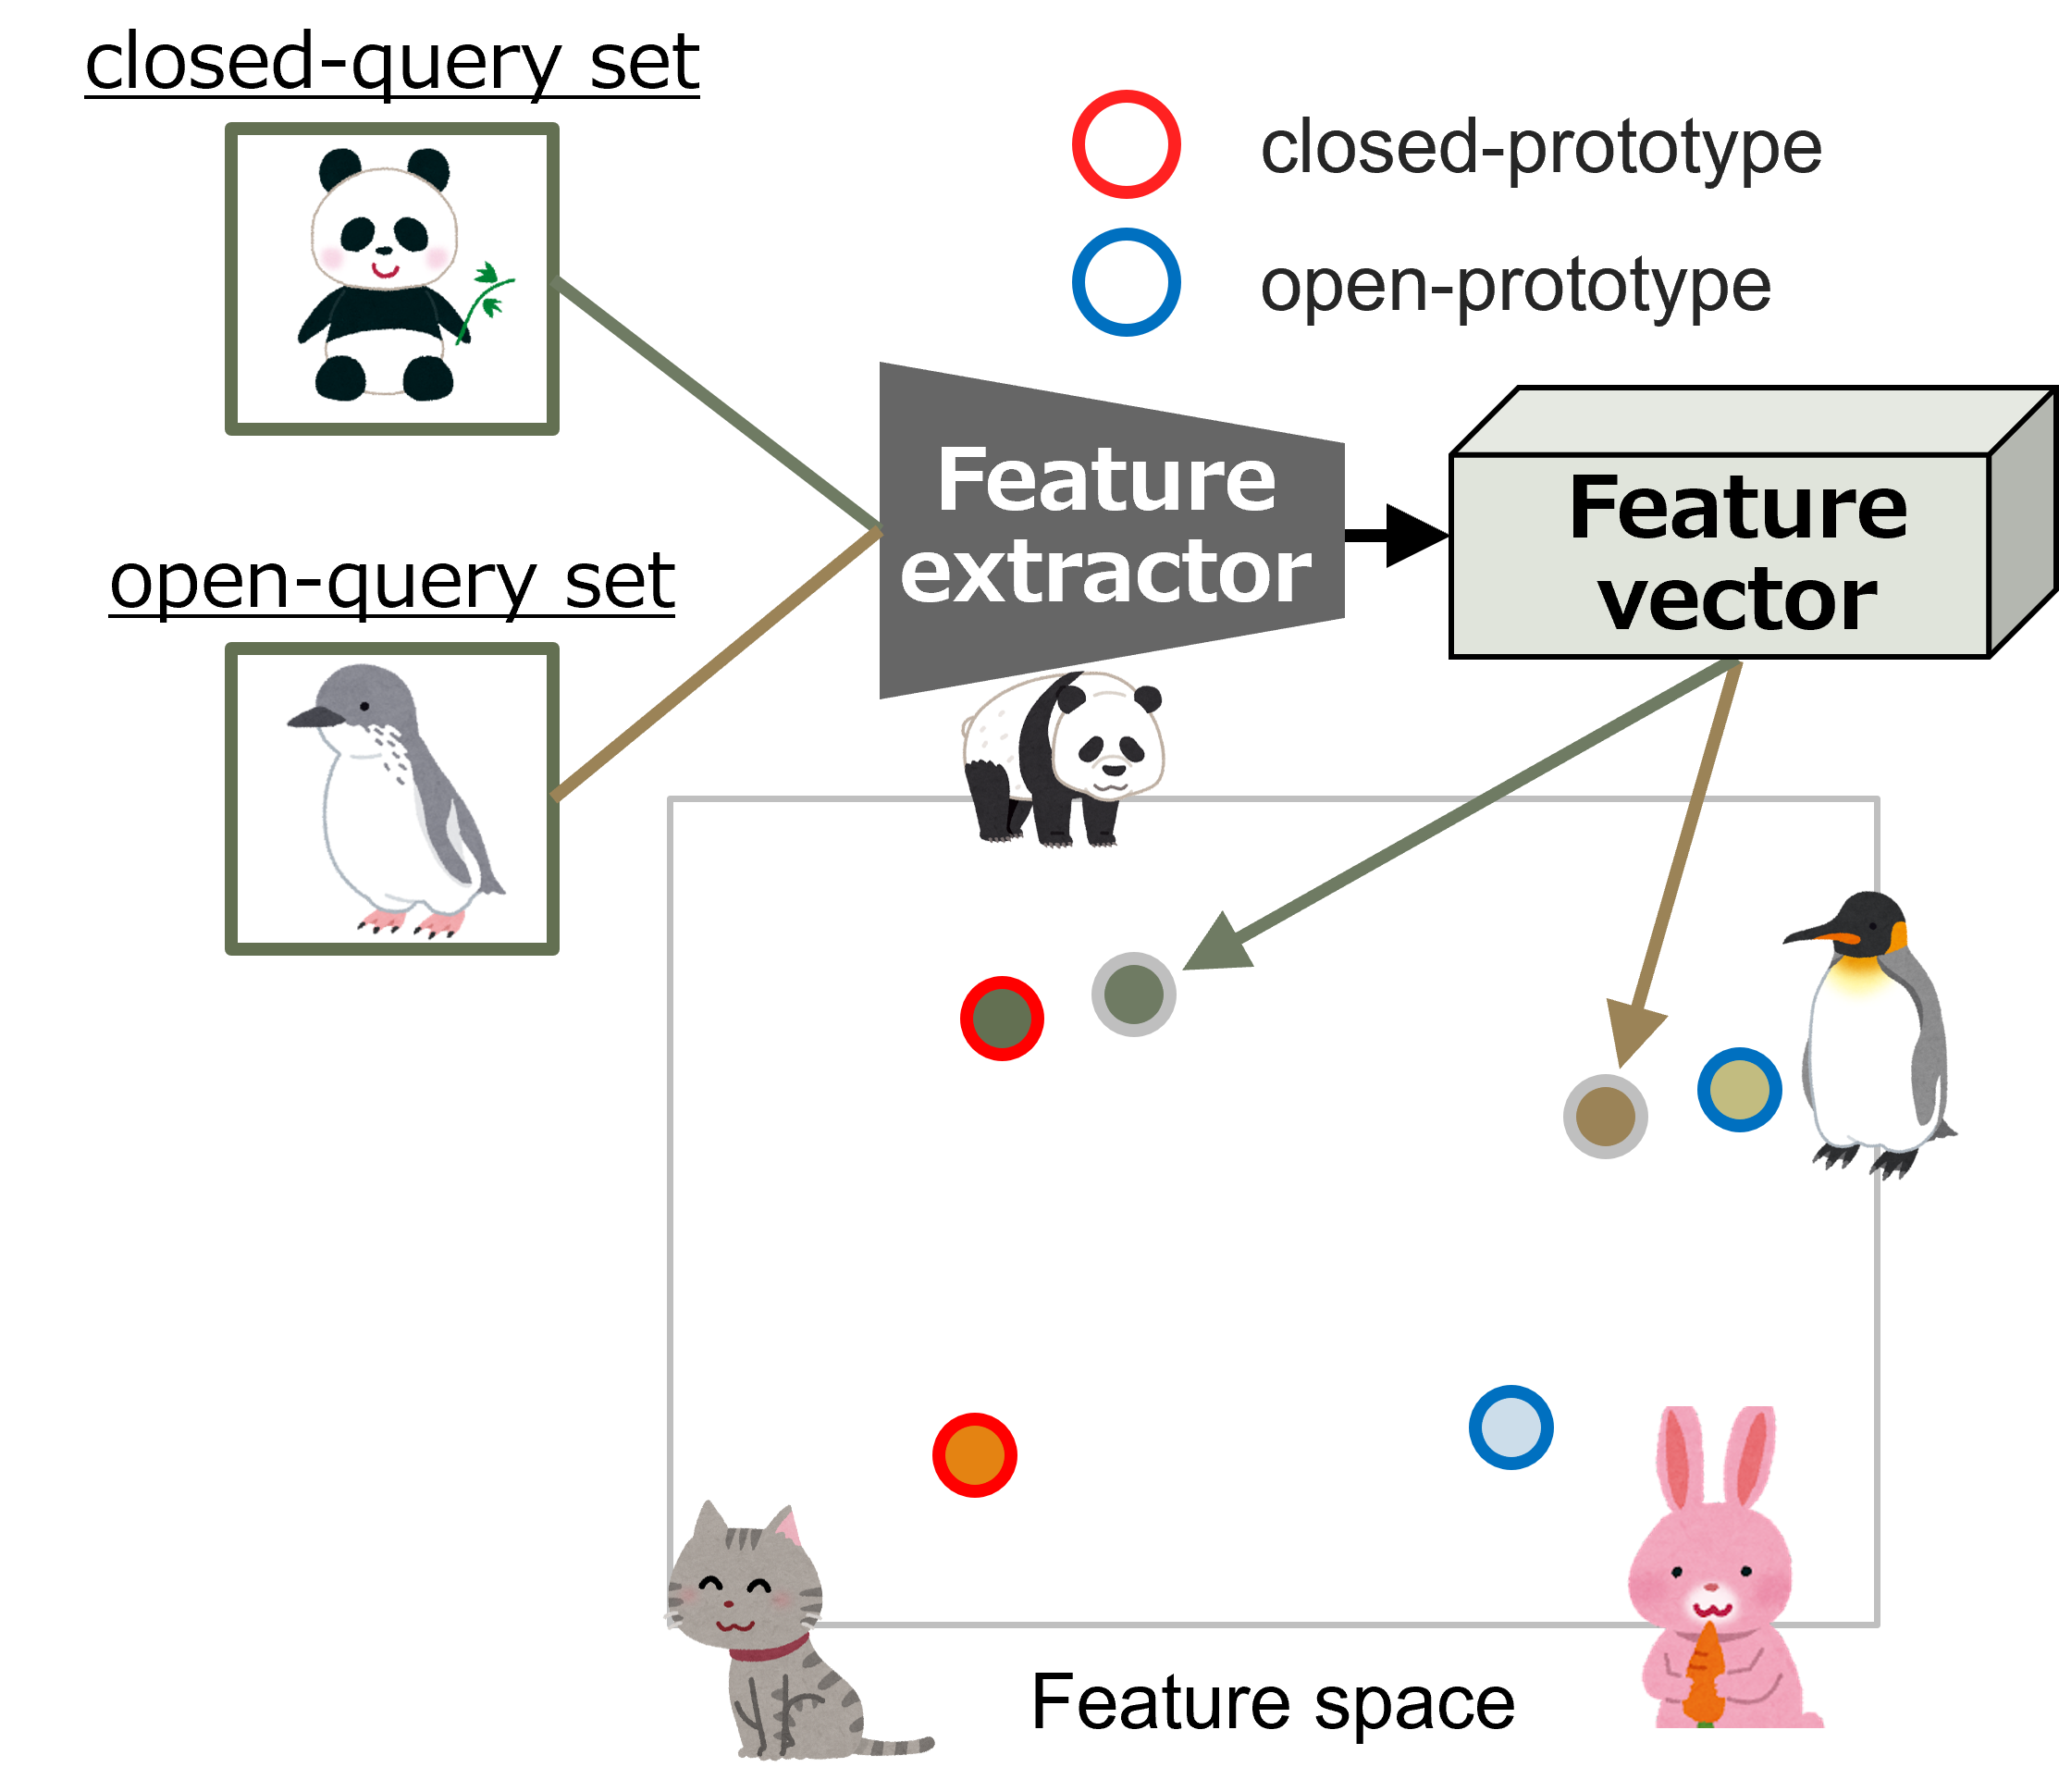
\includegraphics[width=0.8\linewidth, keepaspectratio]{image/open-prototype.png}
  \caption{クローズドプロトタイプとオープンプロトタイプを用いた評価方法}
  \label{fig:openprototype}
\end{figure}
% 
本評価方法においても,特徴抽出器に入力されたクエリセット中の画像は特徴空間上にプロットされ,距離が最も近いプロトタイプのクラスへと分類される.
分類精度は,このようにしてプロトタイプベースの分類が正しく行われた割合に基づき測定される.
ただし,\ref{sec:detect}節とは異なり,クエリデータの特徴点がオープンプロトタイプに近ければそのプロトタイプが属する未登録クラスに分類され,
クローズドプロトタイプに近ければそのプロトタイプが属する登録クラスに分類される.
この評価において,クローズドクエリデータのみの分類精度はClosed Accuracy,オープンクエリデータのみの分類精度はOpen Accuracy,
クローズドクエリデータとオープンクエリデータの分類精度を平均した精度はAll Accuracyとして表される.

本実験の評価設定としても5-Way, 1-Shot問題を採用し,評価用データセットから各エピソードにおいて5つの登録クラスと5つの未登録クラスを選択した.
このうち,クローズドサポートセットとオープンサポートセットには1クラスにつき1枚の画像を選択し,クローズドクエリセットとオープンクエリセットには1クラスにつき15枚の画像を用いて評価を行った.

\subsection{実験結果及び考察}

表 \ref{tbl:exp4}に未登録の動物種の分類結果を示す.
% 
\begin{table*}[tbp]
  \centering
  \renewcommand{\arraystretch}{1.4}
  \caption{IFORにおけるk-means損失とBC損失のアブレーション結果}
  \label{tbl:exp4}
  % \footnotesize
  \small
  \setlength{\tabcolsep}{4pt} % 列幅のパディングをdefaltの6ptから4ptに変更
  \begin{tabular}{c||c|c||c|c|c|c} \hline
    学習フレームワーク                                        &    k-means   &      BC      & Closed Accuracy (\%) & Open Accuracy (\%) & All Accuracy (\%) &      AUROC     \\ \hline\hline
    \multirow{4}{*}{PEELER}                                &              &              &         38.3         &        37.8        &        38.1       & \textbf{49.7} \\ \cline{2-7}
                                                           & $\checkmark$ &              &         38.3         &        37.8        &        38.1       & \textbf{49.7} \\ \cline{2-7}
                                                           &              & $\checkmark$ &         38.3         &        37.8        &        38.1       & \textbf{49.7} \\ \cline{2-7}
                                                           & $\checkmark$ & $\checkmark$ &         39.0         &        38.3        &        38.7       &      49.6     \\ \hline
    \multirow{3}{*}{\shortstack[c]{PEELER\\(w/o 分類損失)}} & $\checkmark$ &              &         39.3         &    \textbf{39.2}   &        39.2       &      49.6     \\ \cline{2-7}
                                                           &              & $\checkmark$ &     \textbf{39.5}    &    \textbf{39.2}   &    \textbf{39.3}  &      49.6     \\ \cline{2-7}
                                                           & $\checkmark$ & $\checkmark$ &         39.3         &    \textbf{39.2}   &        39.2       &      49.6     \\ \hline
  \end{tabular}
\end{table*}
% 
本実験では,距離学習に基づくFSL損失とOSR損失に加え,分類損失を組み合わせた既存のPEELERフレームワークをベースラインとし,k-means損失,BC損失の有効性について検証を行った.
また,全ての実験において,PyTorch Image Models (timm)ライブラリ \cite{timm}によって提供される,
ImageNetで事前学習済みのViTモデル \texttt{deit\_tiny\_patch16\_224}を特徴抽出器として用いた.

結果より,既存手法のPEELERにk-means損失,または,BC損失を個別に組み合わせた場合,モデルの分類精度はベースラインとほぼ同等の性能であった.
一方,k-means損失とBC損失の両方をベースラインのPEELERに組み合わせることによって,ベースラインより高い性能を達成することが確認された.
次に,分類損失を用いないPEELERにk-means損失及びBC損失を組み合わせた結果を確認すると,k-means損失のみ,BC損失のみ,
k-means損失及びBC損失を組み合わせた場合のいずれにおいてもベースラインの精度より高くなることが確認された.
この結果は,IFORの5-Way, 1-Shot問題において,分類損失を用いずにk-means損失やBC損失を単体で用いることの有効性を示している.

% 表 \ref{tbl:exp4}は,新規地域において1枚の画像のみを用いた学習という極めて厳しい条件下での評価結果である.
% ここから,前節の結果を載せるようにする
% しかし,実運用においては,新規地域で撮影された画像が徐々に蓄積されていくため,学習に利用可能な画像枚数 (サポートセット) は増加していく.
% Fig. 5では,評価時の学習画像数𝐾を変化させた場合の分類精度の推移を示した.

\ref{sec:detect}節の表 \ref{tbl:exp1}, \ref{tbl:exp2}並びに \ref{tbl:exp3},本節の表 \ref{tbl:exp4}に示された結果は,新規地域においてサポートセットとしてわずか1枚の画像のみを使用するという,極めて厳しい条件下で評価されている.
しかし,システムの継続的な運用に伴い,サポートセットとして利用できる画像の数は自然に増加することが期待される.
このような実運用シナリオを考慮し,図 \ref{fig:k-shot}に示すように,評価時のShot数$K$が分類精度とAUROCに与える影響ついて検証を行った.
% 
\begin{figure}[tbp]
  \centering
  \begin{subfigure}[b]{0.45\linewidth}
    \centering
    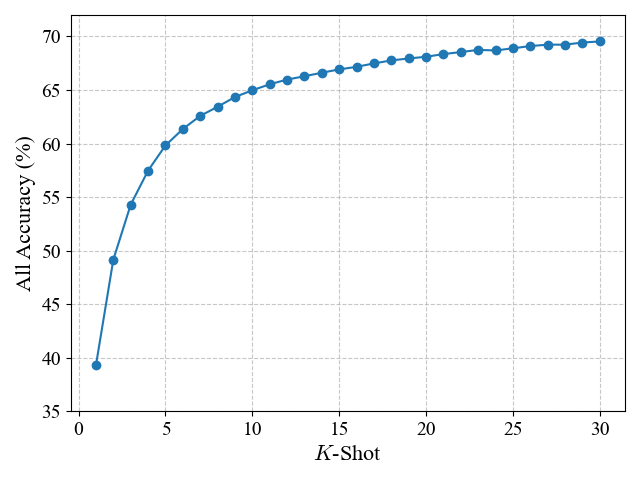
\includegraphics[height=0.9\linewidth, keepaspectratio]{image/sec2k-shotVSaccuracy.png}
    \caption{All Accuracyの推移}
    \label{fig:sec2Accuracy}
  \end{subfigure}
  \hfill
  \begin{subfigure}[b]{0.45\linewidth}
    \centering
    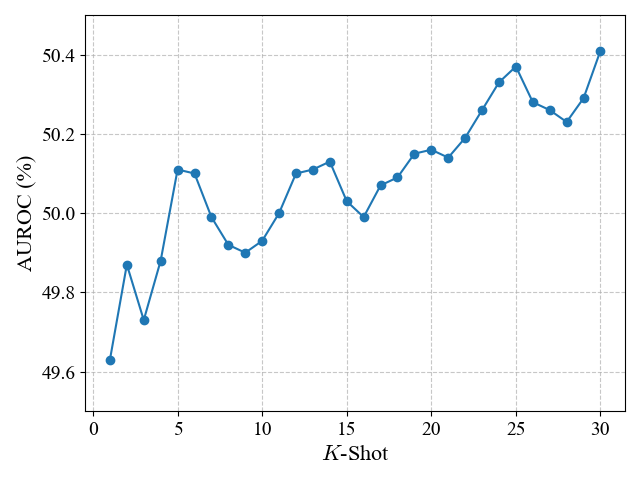
\includegraphics[height=0.9\linewidth, keepaspectratio]{image/sec2k-shotVSAUROC.png}
    \caption{AUROCの推移}
    \label{fig:sec2AUROC}
  \end{subfigure}
  \caption{評価時におけるサポートデータ数$K$が変化した際のAll AccuracyとAUROC}
  \label{fig:k-shot}
\end{figure}
% 
% 本評価では,特徴抽出器としてViT,転移学習手法としてImageNet,学習方法としてメタ学習を採用したモデルを使用した.
% 実験の結果,1クラスあたりの登録データの数を10枚,すなわち,10-shotとすることで,分類精度が75\%を超えることが確認された.
この評価では,特徴抽出器としてViT,転移学習手法としてImageNet,学習方法としてメタ学習,損失関数としてFSL損失,OSR損失,BC損失を採用したモデルを使用した.
実験の結果,図 \ref{fig:sec2Accuracy}に示すように,1クラスあたりのサポートデータを30枚,すなわち,30-Shotまで増加させることによって分類精度が約70\%に達することを確認した.
また,表 \ref{tbl:shot}に各カテゴリーにおける分類精度を示す.

% 表を修正する
\begin{table}[tbp]
  \centering
  \caption{サポートデータのShot数が変化した際の各カテゴリの分類精度}
  \label{tbl:shot}
  \begin{tabular}{c||c|c|c|c|c}
      \hline
      動物種        & 1-shot & 5-shot & 10-shot & 20-shot & 30-shot \\ \hline\hline
      bird         & 26.1   & 49.2   & 55.4    & 58.9    & 60.1    \\
      bobcat       & 36.7   & 55.7   & 59.8    & 61.6    & 64.7    \\
      cat          & 19.4   & 34.5   & 40.9    & 46.6    & 50.5    \\
      coyote       & 25.8   & 41.0   & 47.9    & 53.1    & 54.5    \\
      deer         & 55.4   & 81.9   & 86.1    & 88.0    & 88.1    \\
      dog          & 29.6   & 55.1   & 62.7    & 67.0    & 67.5    \\
      fox          & 34.3   & 47.7   & 54.3    & 58.9    & 60.7    \\
      opossum      & 47.2   & 70.1   & 75.5    & 79.1    & 80.6    \\
      rabbit       & 36.2   & 59.0   & 64.5    & 66.7    & 68.2    \\
      skunk        & 64.3   & 83.5   & 85.6    & 86.3    & 86.9    \\
      squirrel     & 56.7   & 79.1   & 80.9    & 81.6    & 81.9    \\ \hline\hline
      All Accuracy & 39.2   & 59.7   & 64.9    & 68.0    & 69.4    \\ \hline
  \end{tabular}
\end{table}

各実験結果の詳細な分析により,本研究における主要な課題として動物の姿勢による誤分類が明らかとなった.
特に,動物の背面のみが撮影された画像や複雑な姿勢をとる個体の画像など,出現頻度の低い姿勢パターンに対して分類精度の低下が観察された.
図 \ref{fig:animalback}は,このような姿勢の影響により誤分類された画像の具体的な事例を示している.
この課題に対する実用的な解決策としては,カメラトラップにより連続的に撮影された画像群をシーケンスデータとして扱うアプローチが有効である.
複数の連続画像における時間的文脈を考慮することにより,単一の画像からでは判断が困難な姿勢に対しても高精度な分類が期待できる.
この改善案は,モデルの頑健性及び実環境における適用可能性の向上に寄与しつつ,IFORフレームワークの本質的な利点を維持することが可能である.

\begin{figure}[tbp]
  \centering
  \begin{subfigure}[b]{0.45\linewidth}
    \centering
    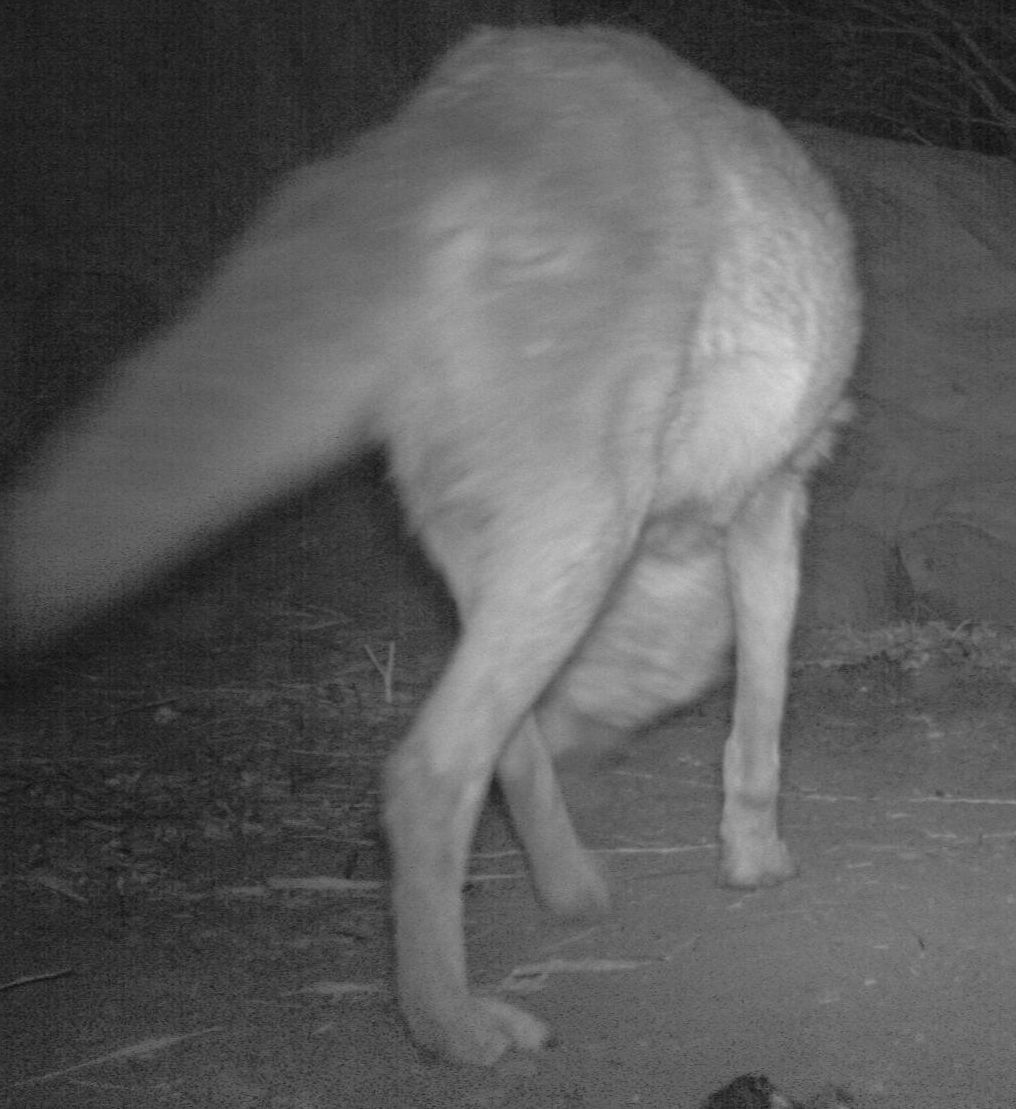
\includegraphics[height=0.9\linewidth, keepaspectratio]{image/coyote.png}
    \caption{coyoteの画像例}
    \label{fig:coyote}
  \end{subfigure}
  \hfill
  \begin{subfigure}[b]{0.45\linewidth}
    \centering
    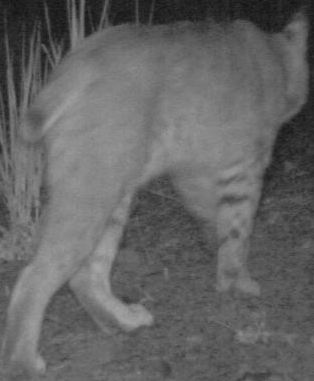
\includegraphics[height=0.9\linewidth, keepaspectratio]{image/bobcat.png}
    \caption{bobcatの画像例}
    \label{fig:bobcat}
  \end{subfigure}
  \caption{姿勢が原因で誤分類された画像例(正解カテゴリ: coyote, 予測カテゴリ: bobcat)}
  \label{fig:animalback}
\end{figure}